%-------------------------------------------------------------------------------------------
	\section{Heighway dragon oritatami system}
%-------------------------------------------------------------------------------------------

We propose a generic design of deterministic oritatami system that allows us to fold an arbitrary finite portion of the Heighway dragon. 
The design concept has been already explained in the introduction. 
The dragon it folds into is actually slanted as illustrated in Figure~\ref{fig:heighway6_oritatami}, which is more natural than the conventional (upright) one to be folded over the triangular grid. 
The design sets both delay and arity to 3 and employs a fixed number of bead types (about 2000), no matter which portion is folded. 
Minimizing the number of bead types has just proven NP-hard \cite{HanKim2017}. 

Any finite portion of the Heighway dragon is expected to be foldable by \textit{hard-coding} if an arbitrary number of bead types is available and the shape can be scaled-up (though, if rescaling is not allowed, it is NP-hard to decide if for a given finite shape, there exists an oritatami system that folds into the shape \cite{PatitzRogers2017}). 
The proposed design cannot take this approach because the number of bead types available is fixed. 
An oritatami system $\Xi = (\mathcal{H}, \alpha, \delta, \sigma, w)$ that the design provides is periodic in the sense that its transcript is a periodic sequence. 
If this system is for the $n$-th repetition of the Heighway dragon, then the length of its period is $|w|/2^{n-1}$. 
One period corresponds to a successive two pairs of a red line segment and the following green L-shaped block. 

Why do these two pairs have to be distinguished from each other? 
The answer to this question lies in the fact that the Heighway dragon is slanted. 
The slanted dragon involves two types of left turn as well as two types of right turn: acute and obtuse. 
Capability of one turning module to make all of the four possible turns would shorten the period by half. 
Such a turning module, however, would have to take quite a large number of conformations; recall that what the module has to turn is not a straw but a thick wire which bears the current count $i$. 
Implementing such a module totally ignores the level of oritatami design techniques accumulated so far.  
Our approach makes it sufficient to implement a turning module capable of just an acute turn and an obtuse turn. 
Observe that after the (slanted) vertical segment, certainly the left turn is obtuse while the right turn is acute, whereas after the horizontal segment, the left turn is acute while the right turn is obtuse. 
In addition, we know \textit{a priori} which segments are vertical and which are horizontal; indeed vertical segments and horizontal segments occur alternately on the Heighway dragon. 
Therefore, we can attach a proper interpreter to a DFAO module to convert its output L/R into a signal A(cute)/O(btuse). 
Two types of interpreters are hence needed: vertical interpreter converts L into obtuse and R into acute, while horizontal one converts them the other way around. 

\begin{figure}[h]
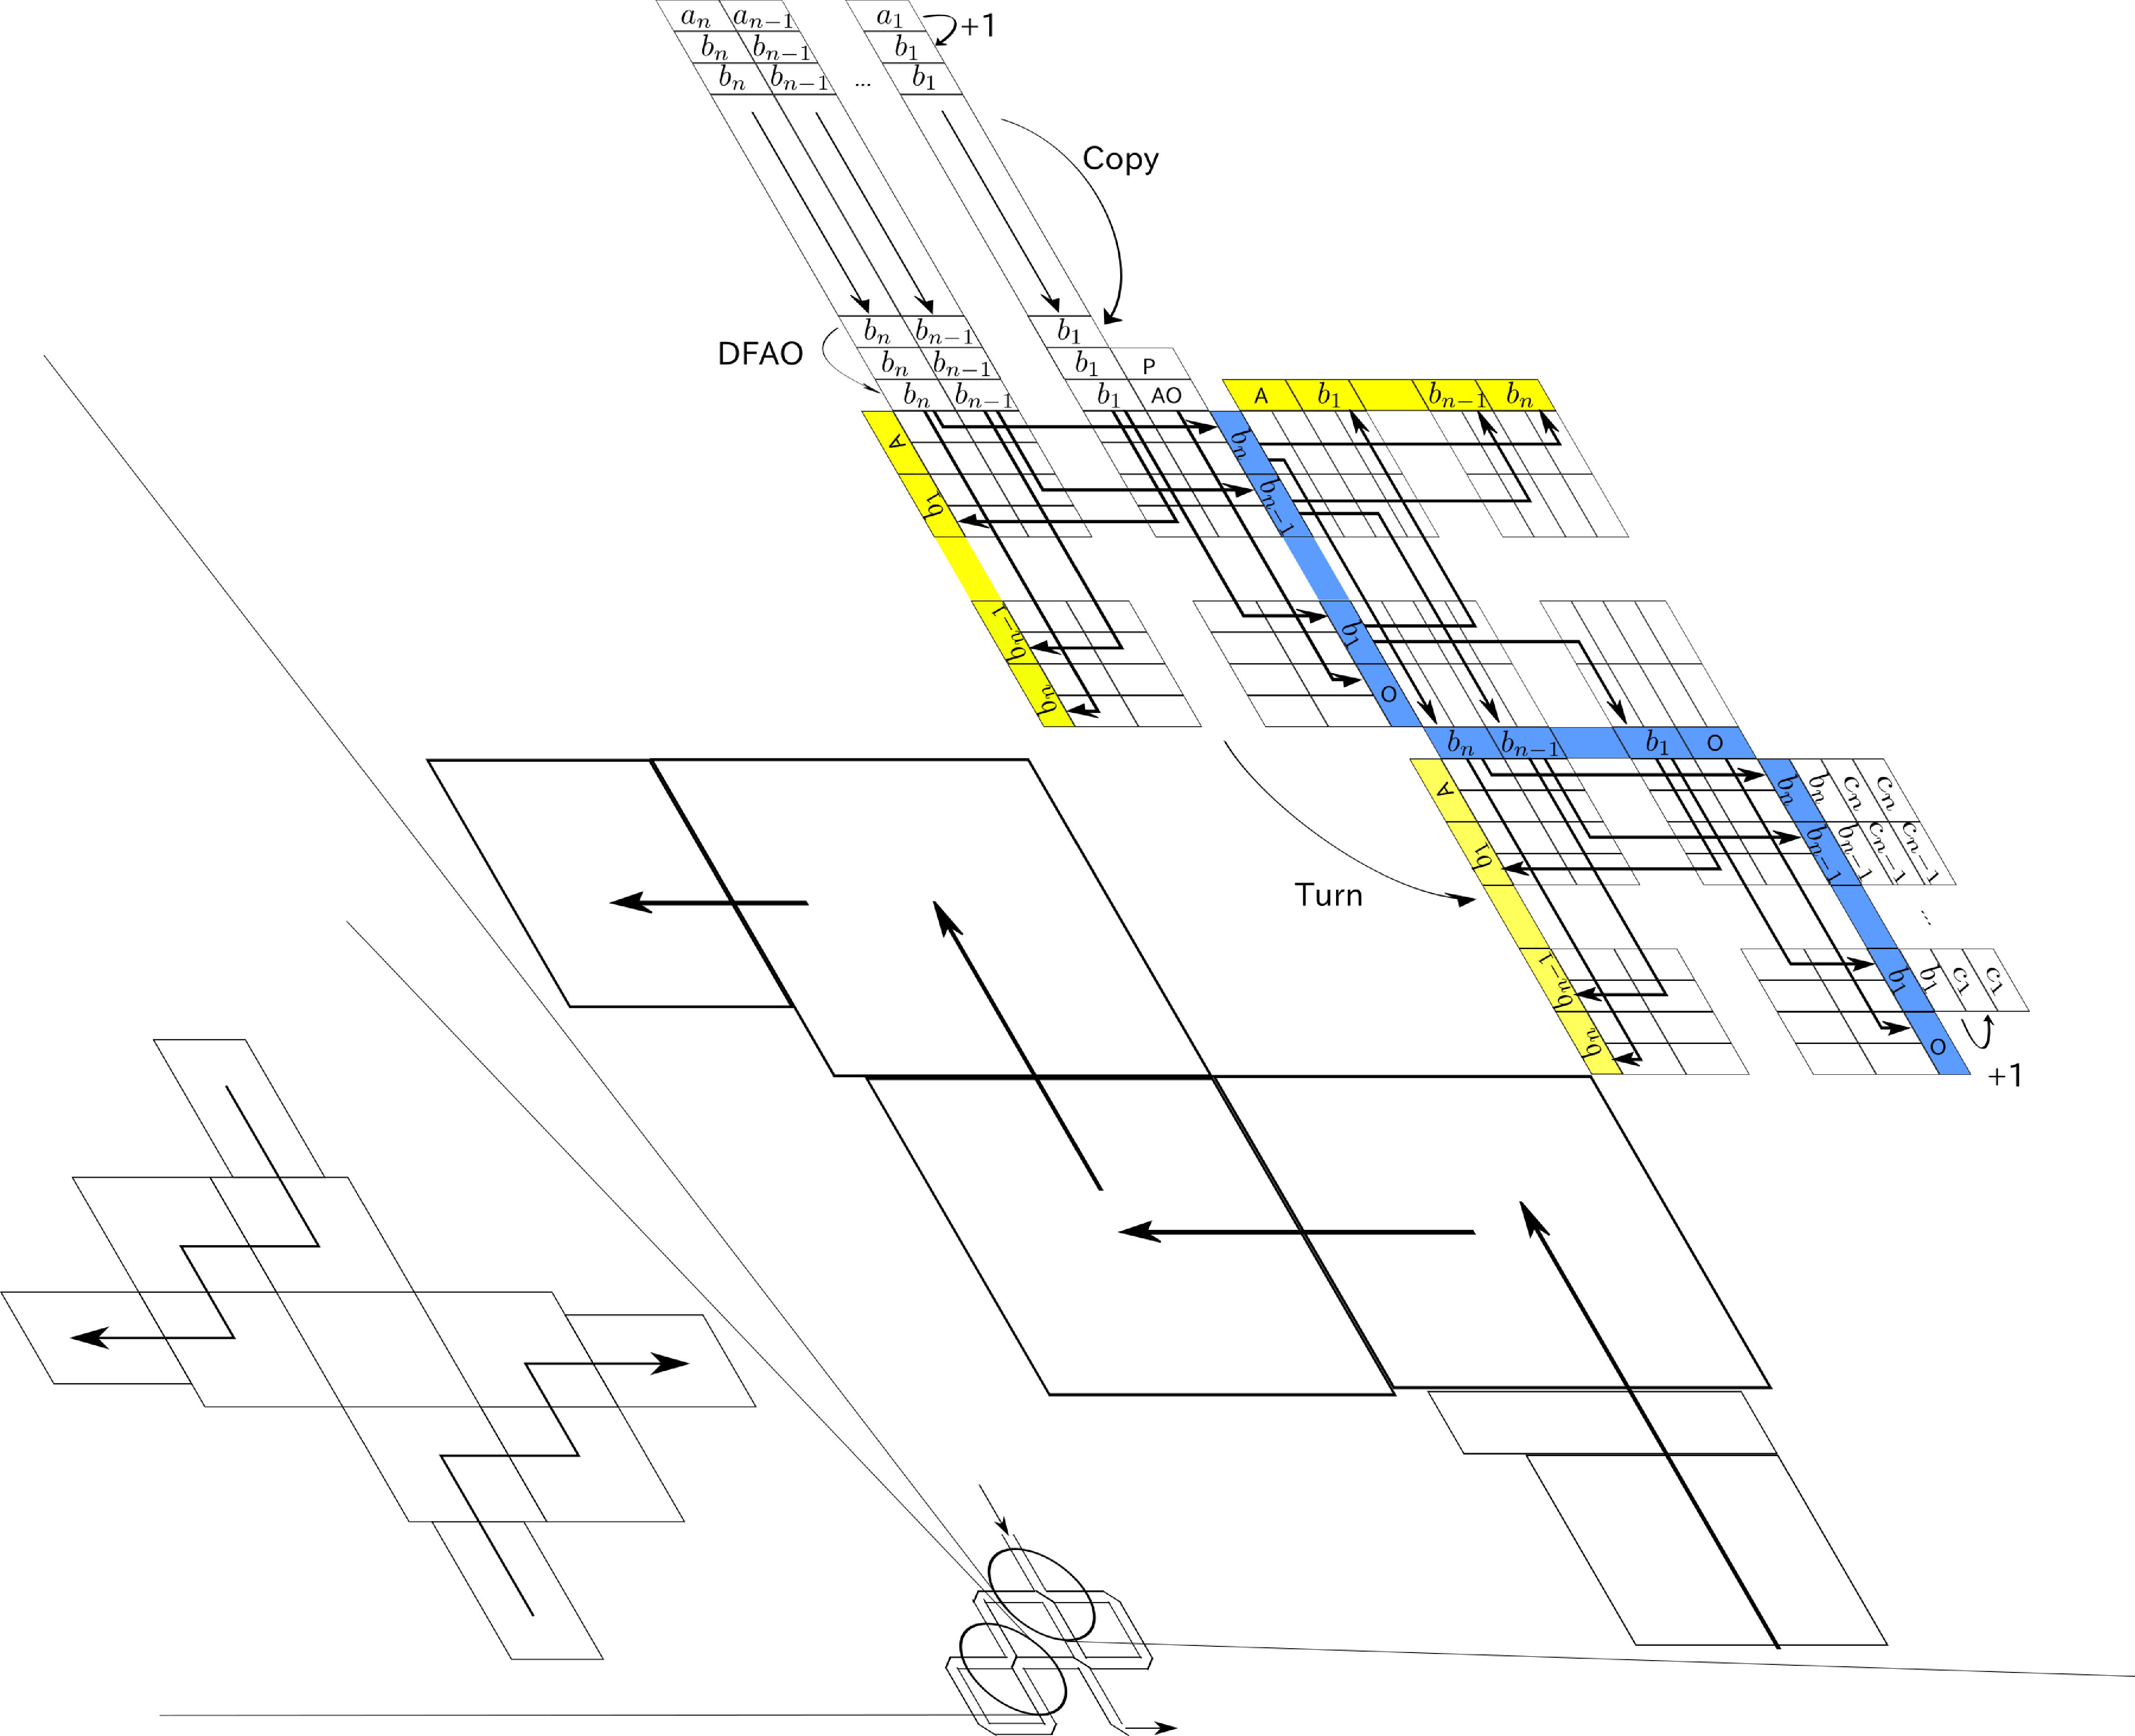
\includegraphics[width=\linewidth]{pic/dragon_vol4.pdf}
\caption{
Folding of one segment plus turn of the Heighway dragon, flow of information through it, and two ways of collision avoidance between two turns.
}
\label{fig:abst_dragon}
\end{figure}

The sole difference between the first and second halves of a period is anyway the type of interpreter (AO or $\overline{\rm AO}$). 
Thus, it should be sufficient to explain only the first half. 
The half consists of four subsequences for the counter, copier, DFAO, and turning modules. 
It folds as abstracted in Figure~\ref{fig:abst_dragon} into one line segment plus one turn of the Heighway dragon and has its four modules accomplish the following processes, respectively: 
\begin{enumerate}[itemsep=0pt]
\item $i \gets i + 1$ (count-up)
\item Copy $i$ (drawing a line segment)
\item Compute $P[i]$
\item Make a turn according to $P[i]$
\end{enumerate}
Its length is proportional to $n^2$ and hence so is the length of a period. 
The seed of the system replaces the counter module at the beginning of the first period and encodes the initial value of $i$ as a sequence of bead types in an appropriate format such that copier modules can ``read'' the count $i$. 
We shall explain how modules read something in Section~\ref{subsubsec:module_counter}. 
Before explaining the implementation of each module, we should point out one significant issue specific to the folding by oritatami systems. 
It rises when the Heighway dragon makes a turn where it has already made another turn before, that is, when two turns share a point. 
By definition, oritatami systems cannot put a bead anywhere occupied by another bead. 
This is the reason of the L-shape of the turning module. 
As shown in Figures~\ref{fig:heighway6_oritatami} and \ref{fig:abst_dragon}, the proposed system makes an acute turn by having three bifurcation components direct the growth of further folding acutely one after another, while an obtuse turn by having them direct the growth rather obtusely. 

%-------------------------------------------------------------------------------------------
		\subsection{Modules}
%-------------------------------------------------------------------------------------------

Now it suffices to explain how modules and their components are implemented, interlocked with each other, and collaborate. 
Using the simulator developed for \cite{HaKiOtSe2016}, we have verified that all of the components fold correctly in all possible environments, which are abstracted in Figures~\ref{fig:abst_dragon}, \ref{fig:abst_dfao}, and \ref{fig:overall_turning}. 

%-------------------------------------------------------------------------------------------
			\subsubsection{Counter and copier modules}
			\label{subsubsec:module_counter}
%-------------------------------------------------------------------------------------------

The existing binary counter \cite{GeMeScSe2016} was modified so as to operate in the dynamics \eqref{eq:cotranscriptional_folding}, which is more prevailing \cite{GeMeScSe2015,HanKim2017,HaKiOtSe2016,OtaSeki2017} but less tractable than the one the original counter used. 

%%%%%%%%%%%%%%%%%%%%%%%%%%%%%%%%%%%%%%%%%%%%
\begin{figure}[h]
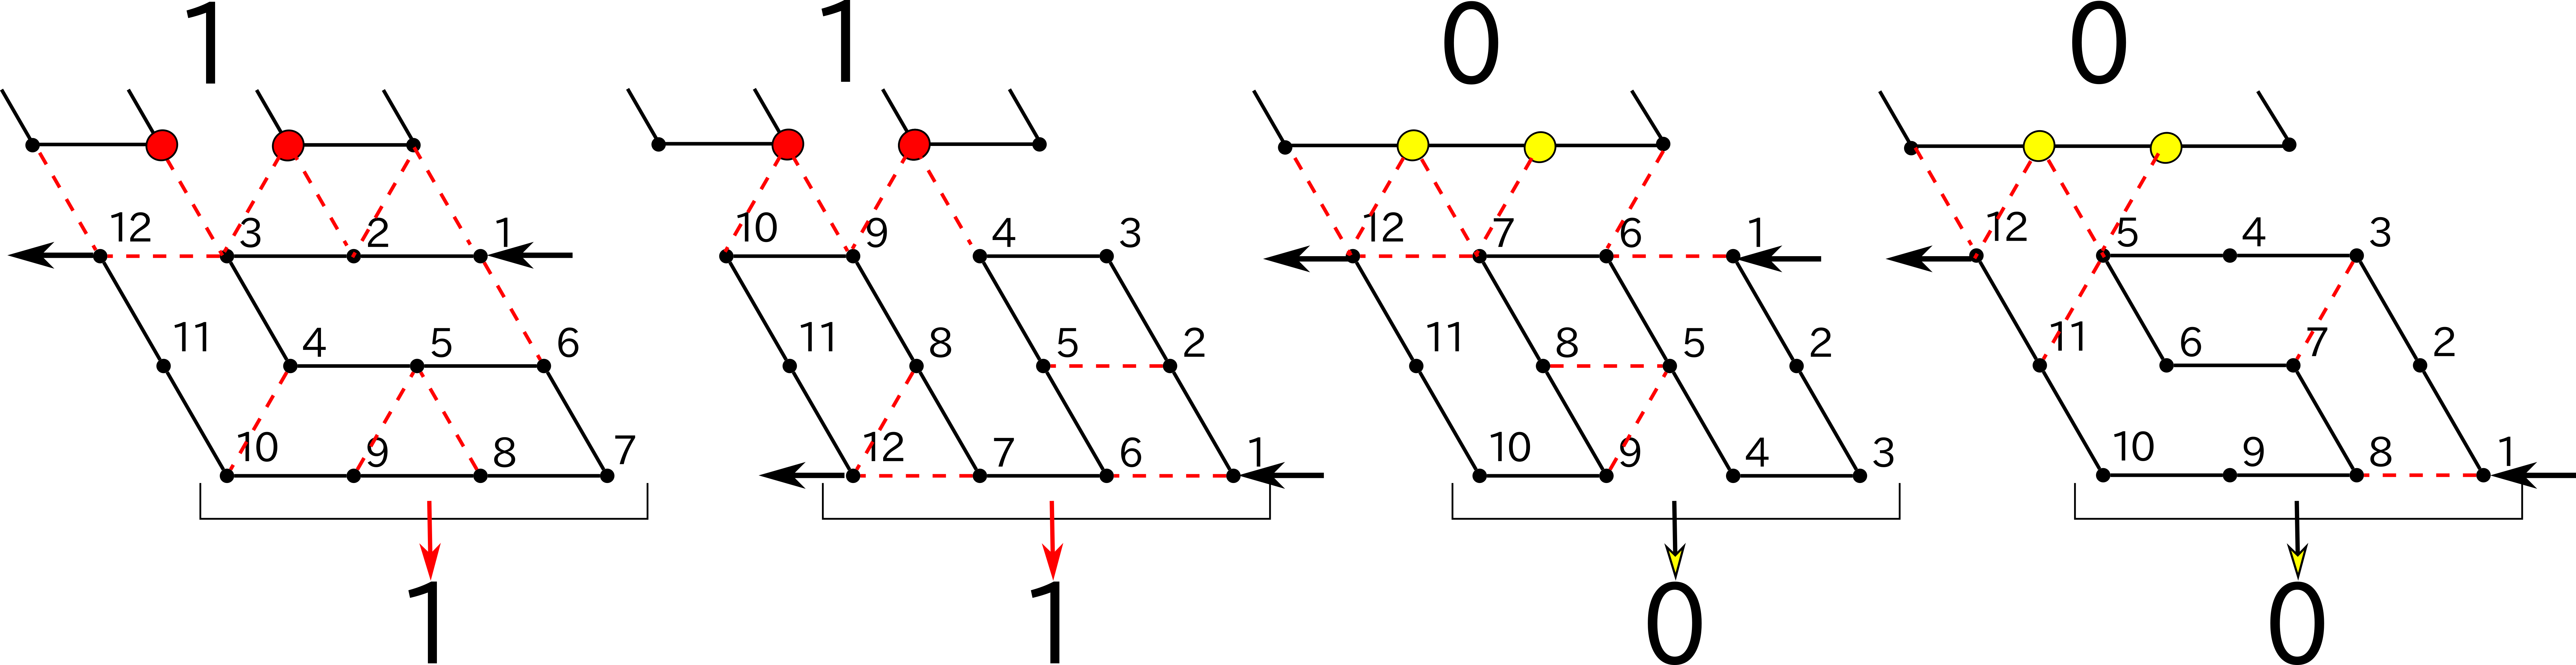
\includegraphics[width=\linewidth]{pic/counter_zig.png}
 \caption{All conformations of the half-adder component.}
\label{fig:half-adder}
\end{figure}
%%%%%%%%%%%%%%%%%%%%%%%%%%%%%%%%%%%%%%%%%%%%

The essential component of this module is the half-adder. 
In Figure~\ref{fig:abst_dragon}, half-adder components are abstracted as small rhombuses at the top labeled with $a_n, a_{n-1}, \ldots, a_1$, where the one with $a_j$ is for the $j$-th bit of the current count $i$. 
Though not described, two horizontally adjacent half-adders sandwitch a glider of even length as a space to keep them away from each other sufficiently to prevent any undesirable interference. 
Figure~\ref{fig:half-adder} illustrates its four possible conformations. 
The whole oritatami system is designed in such a manner that a 1-bit input (1 or 0) is exposed to the specific position (colored red or yellow in Figure~\ref{fig:half-adder}) as a pair of bead types by the previous turning module. 
The system is also designed in such a manner that a half-adder starts folding either at the top, as in the first and third conformations, or at the bottom as in the other two. 
The half-adder considers the top start position as non-carry and the bottom start position as carry. 
Thus, only when a half-adder takes 1 and carry, it ends at the bottom (second conformation in Figure~\ref{fig:half-adder}), which is propagated to the next half-adder as it is via the spacer between them. 
These four conformations expose sequences of four bead types below that are distinct enough to convey the intended 1-bit output to another computing component, or in other words, we can design a component that can ``read'' the output. 
From this point forward, conformations for other components will be illustrated; their input and output will be labeled by their meaning mutually understood by the components that exchange them. 

Being fed with non-carry, the counter module serves as the copier module. 
Combining them one after another yields a line segment of arbitrary length, through which the current count $i$ is propagated. 


%-------------------------------------------------------------------------------------------
			\subsubsection{DFAO module}
%-------------------------------------------------------------------------------------------


A DFAO module receives the current count $i$ from the last copier module, computes $P[i]$, interprets it properly either A or O, and outputs it together with the count $i$ at the very end of a red line segment. 

\begin{figure}[h]
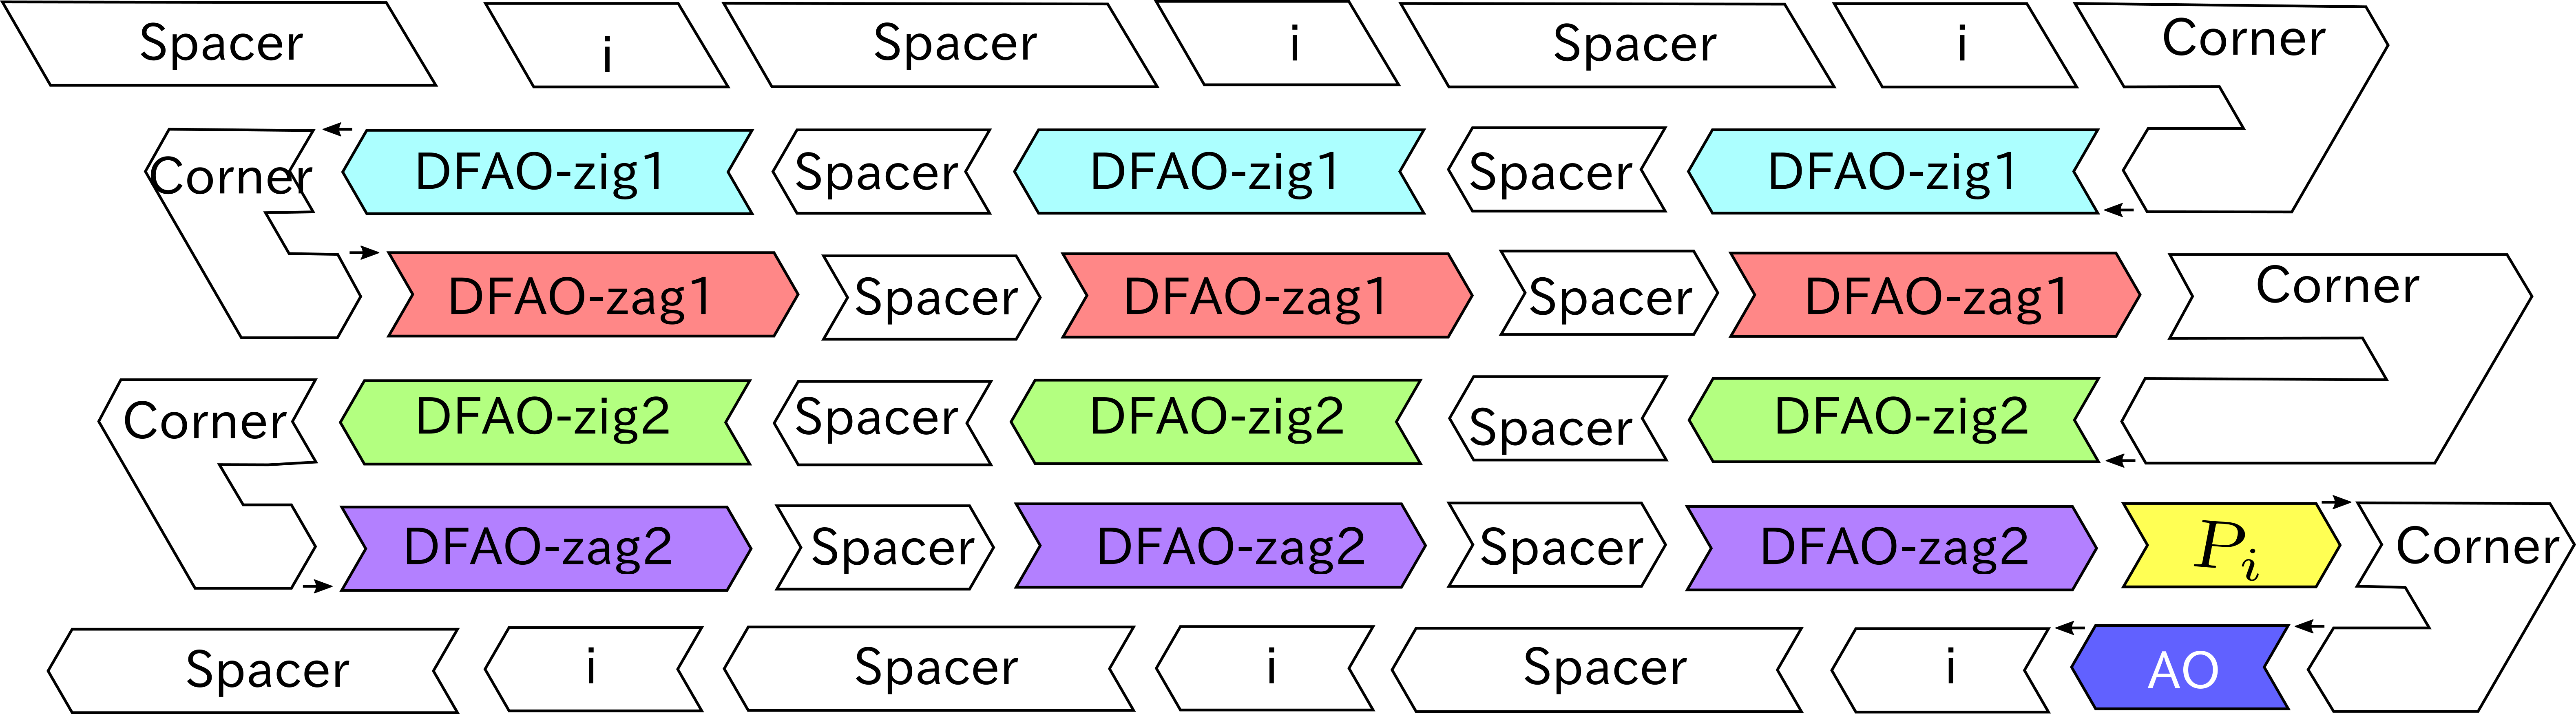
\includegraphics[width=\linewidth]{pic/abst_DFAO.png}
\caption{Component-level abstraction of the folding of DFAO module.}
\label{fig:abst_dfao}
\end{figure}

%%%%%%%%%%%%%%%%%%%%%%%%%%%%%%%%%%%%%%%%%%%%

\begin{figure}[h]
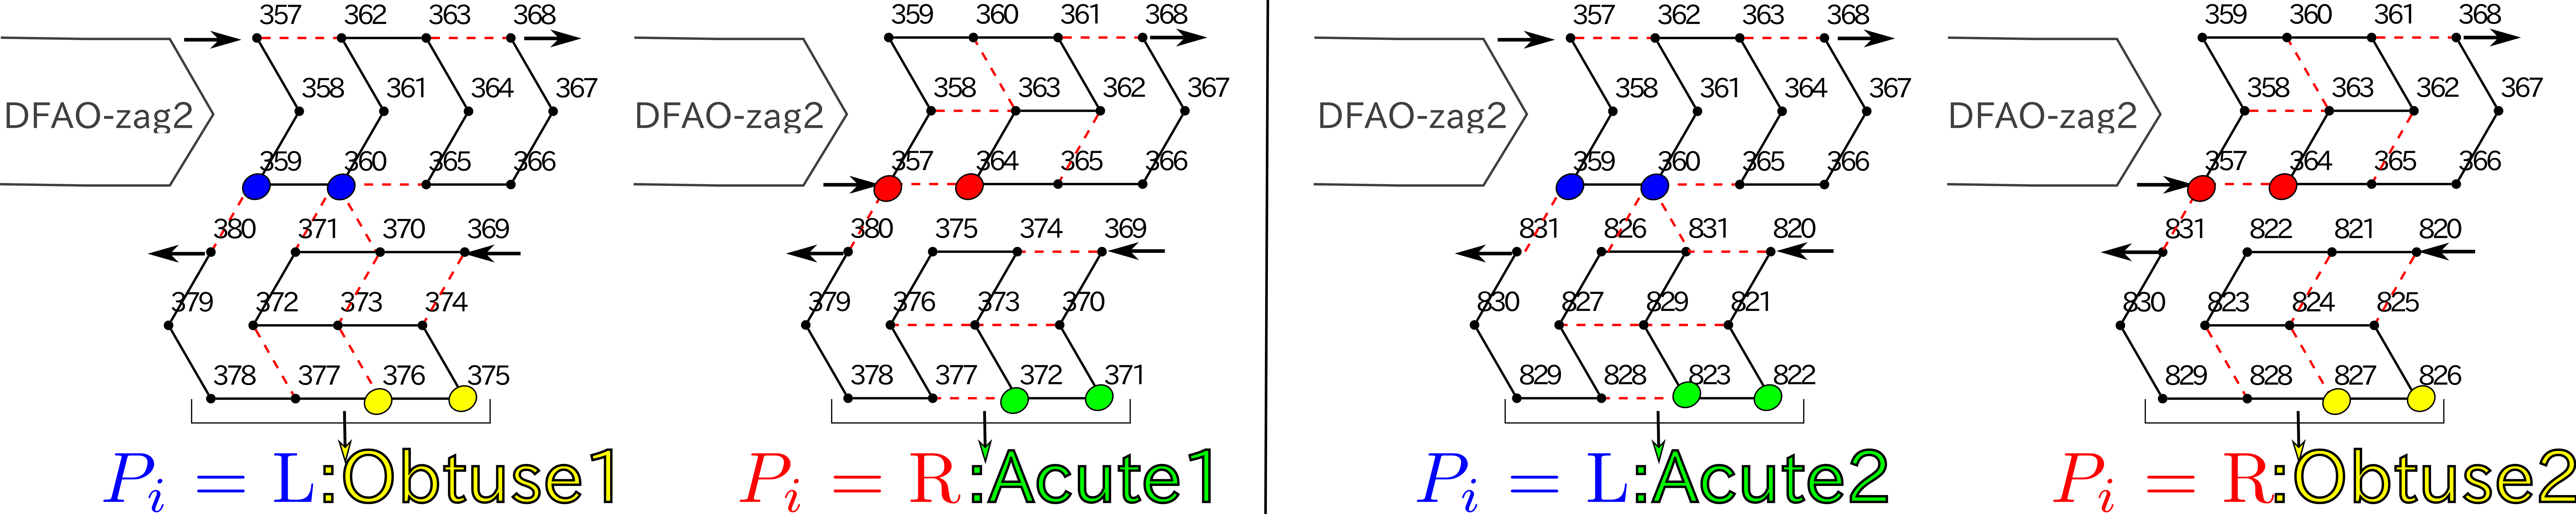
\includegraphics[width=\linewidth]{pic/PFS.png}
\caption{(left) The possible two conformations of PFS: PFS-L, PFS-R. (right) The possible two conformations of AO.}
\label{fig:PFS}
\end{figure}
%%%%%%%%%%%%%%%%%%%%%%%%%%%%%%%%%%%%%%%%%%%%


DFAO is composed of the six components: DFAO-zig, DFAO-zag1, DFAO-zig2, DFAO-zag2, PFS, AO (or  ``$\overline{\rm AO}$").
At the component-level, it folds into two zig-zags as abstracted in Figure~\ref{fig:abst_dfao}.
What the module does in the first zig-zag is to have DFAO-zig1s and DFAO-zag1s read the current count $i$ from its LSB and ``mark" the first 0, while propagating $i$.
In the second zig-zag, it employs DFAO-zig2s and DFAO-zag2s to check whether the automaton transitions to the state $q_2$ ($P_i = L$) or else ($P_i = R$).
The second zag is to end at the top if $P_i = L$ or at the bottom if $P_i = R$.
PFS takes one of the two conformations in Fig.~\ref{fig:PFS} and outputs $P_i$ downward.
In vertical segments, PFS is followed by AO, while in horizontal segments, it is followed by $\overline{\rm AO}$.
AO interprets the PFS' output $P_i = R$ as acute and $P_i = L$ as obtuse, as shown in Fig.~\ref{fig:PFS}.
$\overline{\rm AO}$ interprets them the other way around.
Let us explain briefly how each of the components folds to fulfill its roles.

%%%%%%%%%%%%%%%%%%%%%%%%%%%%%%%%%%%%%%%%%%%%
\begin{figure}[h]
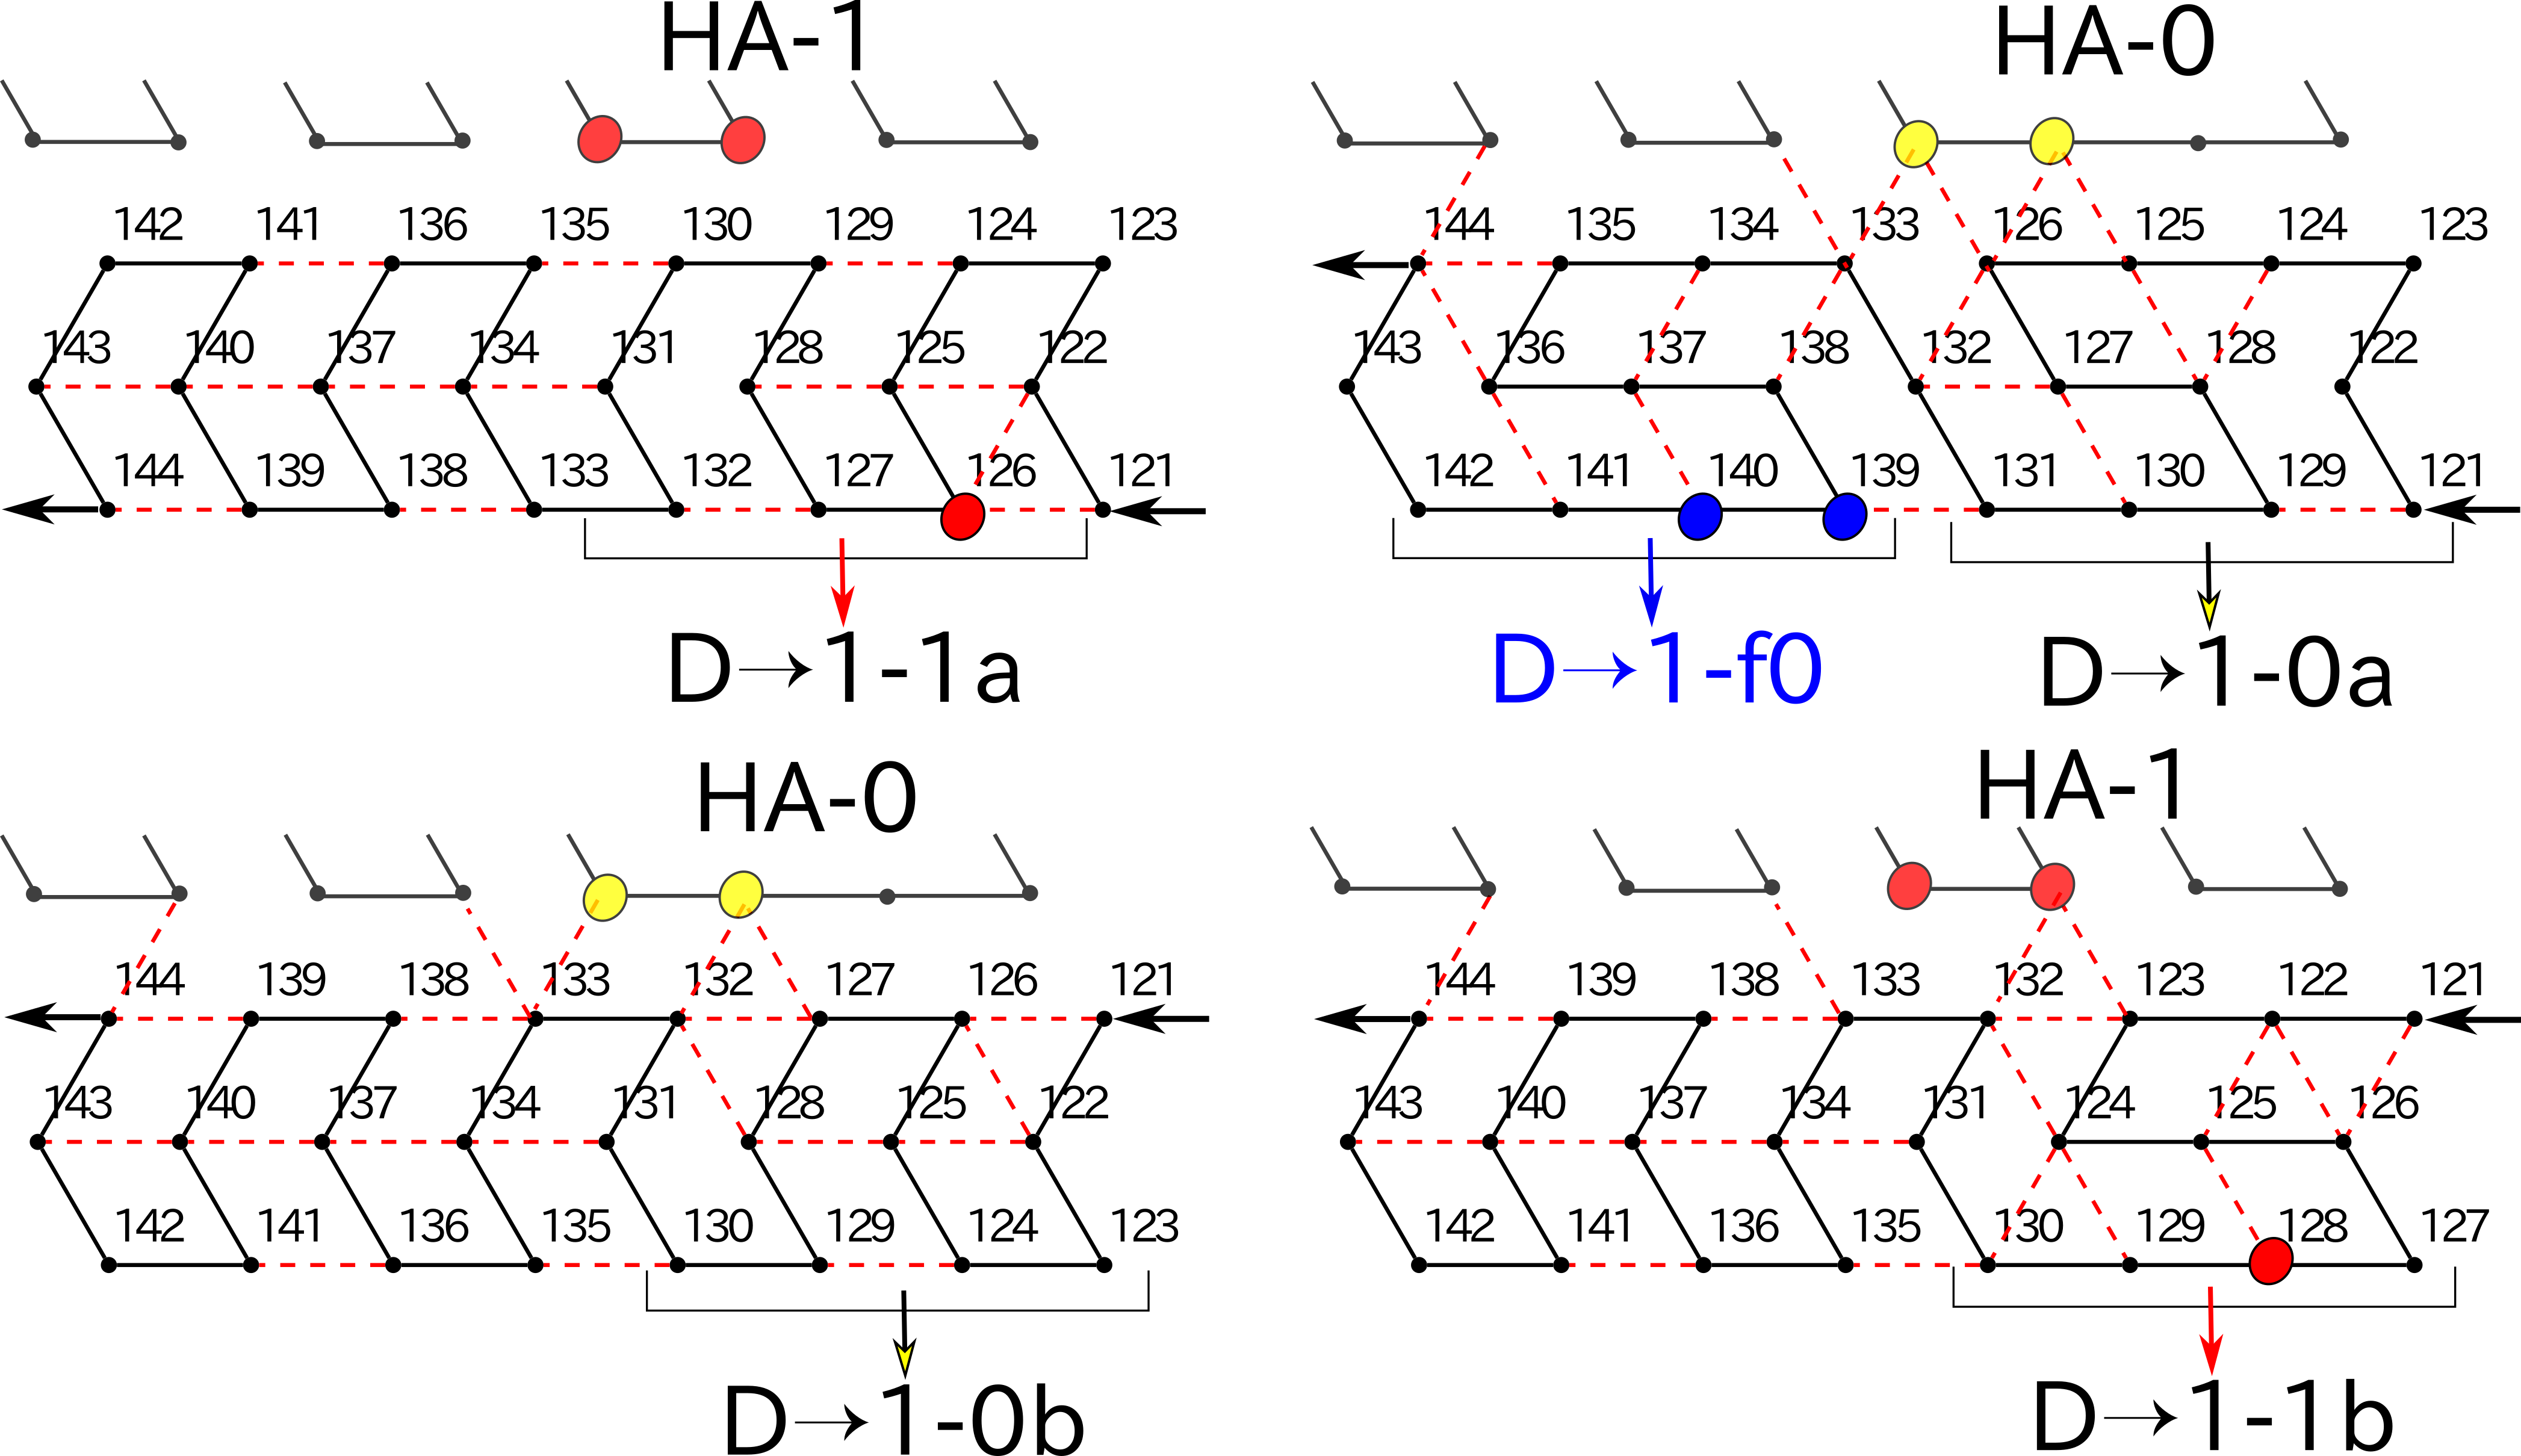
\includegraphics[width=\linewidth]{pic/DFAO-zig1.png}  
  \caption{The possible four conformations of DFAO-zig1: (top) Dzig1-1 and Dzig1-f0; (bottom) Dzig1-20 and Dzig1-21.}
  \label{fig:DFAO-zig1}
\end{figure} 

%%%%%%%%%%%%%%%%%%%%%%%%%%%%%%%%%%%%%%%%%%%%%%%%%%%%

\begin{figure}[h]
  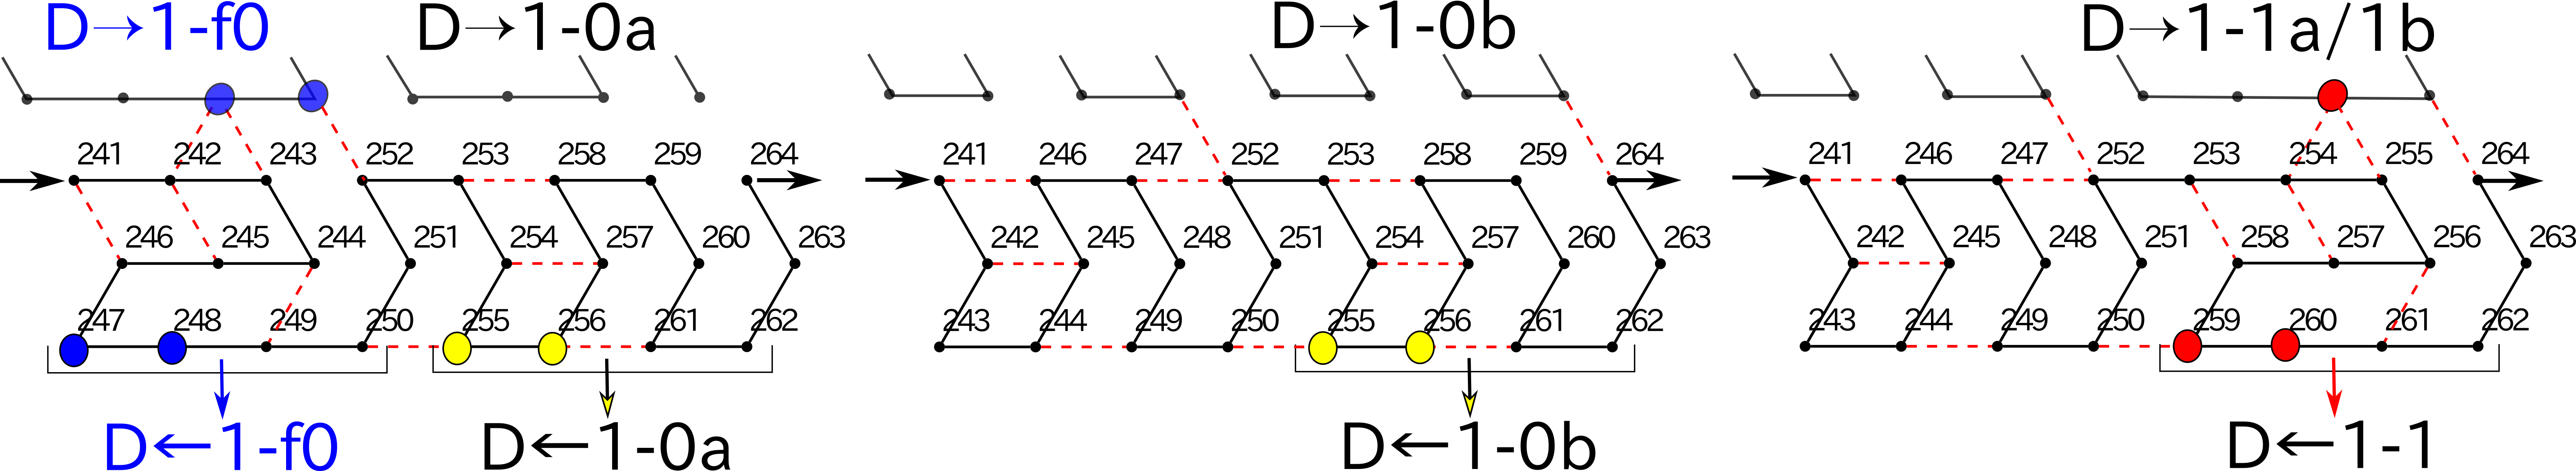
\includegraphics[width=\linewidth]{pic/DFAO-zag1.png}
  \caption{The possible three conformations of DFAO-zag1: Dzag1-f0, Dzag1-0, and Dzag1-1 from left.}
  \label{fig:DFAO-zag1}
\end{figure} 
%%%%%%%%%%

DFAO-zig1's collaboratively detect the first 0 in two phases.
Phase1 is to copy all the 1's before the first 0 and Phase2 is to copy all the bits after the first 0.
These phases are distinguished by the relative position at which a DFAO-zig1 starts folding to the copier above (in Phase1 it is at the bottom, while in Phase2 it is at the top, as suggested in Figure~\ref{fig:DFAO-zig1}).
In Phase1, DFAO-zig1s certainly take the conformation Dzig1-1 (the top left conformation in Figure~\ref{fig:DFAO-zig1}).
In Phase1, if the half-adder above outputs 0, this is the first 0. 
Then the DFAO-zig1 takes the conformation Dzig1-f0 instead, ending at the top to transition to Phase 2.
Each of the succeeding DFAO-zig1s takes one of the other two conformations Dzig1-20 and Dzig1-21 to copy all the remaining bits. 
Note that there is a cushion between two DFAO-zig1s called \textit{spacer}.
Spacers have been already used to prevent undesirable interference among components.
They are implemented as a glider (see Example~\ref{ex:glider}), hence capable of propagating 1bit on which phase the system is in.
In the first zag, DFAO-zag1's just propagate 0's, 1's, and the first 0 by taking the proper one of the three conformations in Figure~\ref{fig:DFAO-zag1}.

%%%%%%%%%%%%%%%%%%%%%%%%%%%%%%%%%%%%%%%%%%%%
\begin{figure}[h]
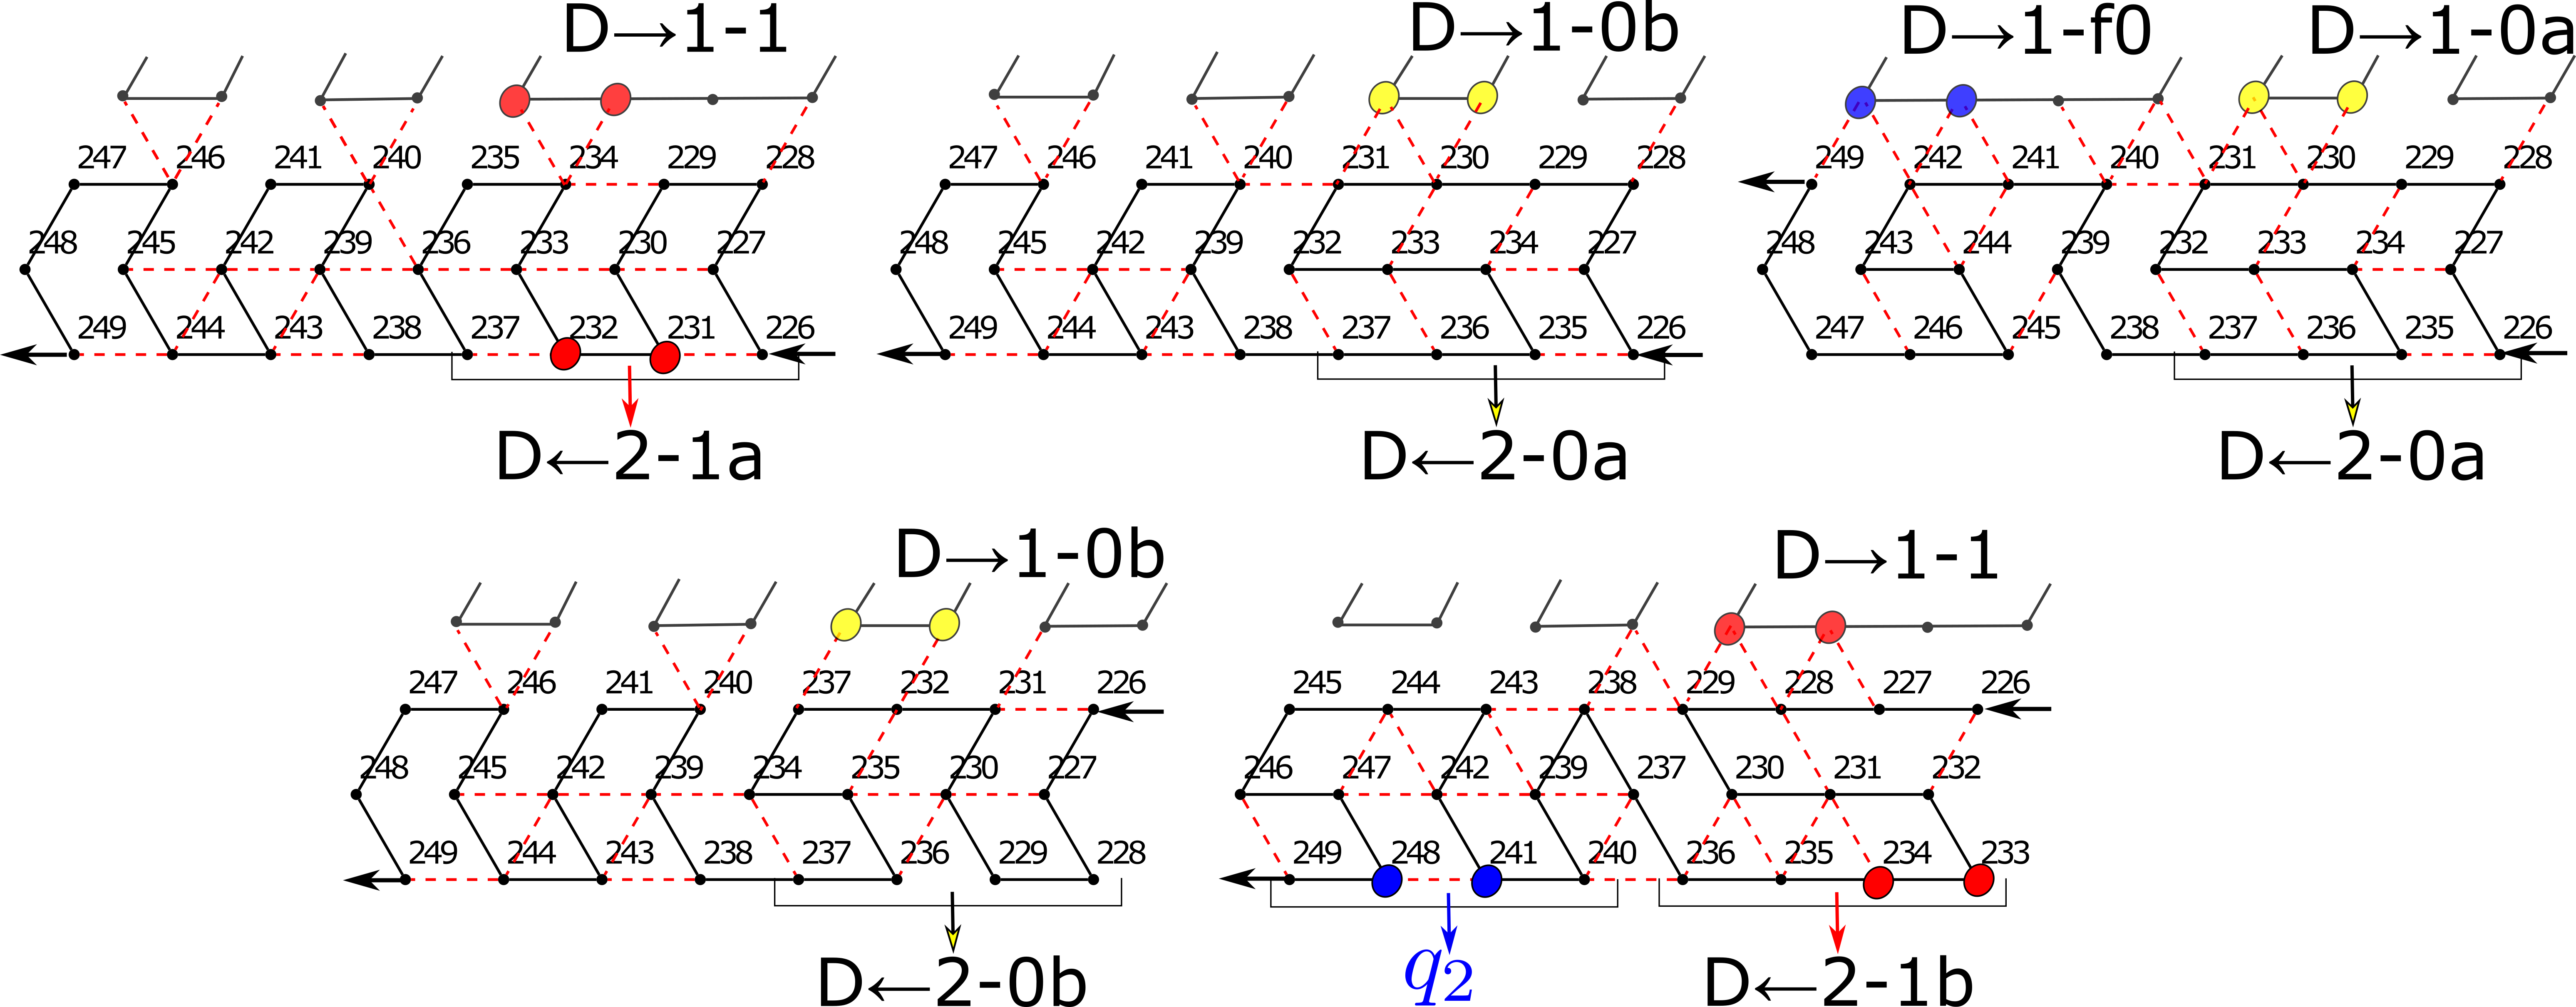
\includegraphics[width=\linewidth]{pic/DFAO-zig2.png}
  \caption{The possible five conformations of DFAO-zig2: (top) Dzig2-1, Dzig2-0, Dzig2-f0, (bottom) Dzig2-f00, and Dzig2-f01. }
  \label{fig:DFAO-zig2}
\end{figure} 

%%%%%%%%%%%%%%%%%%%%%%%%%%%%%%%%%%%%%%%%%%%%%%%%
\begin{figure}[h]
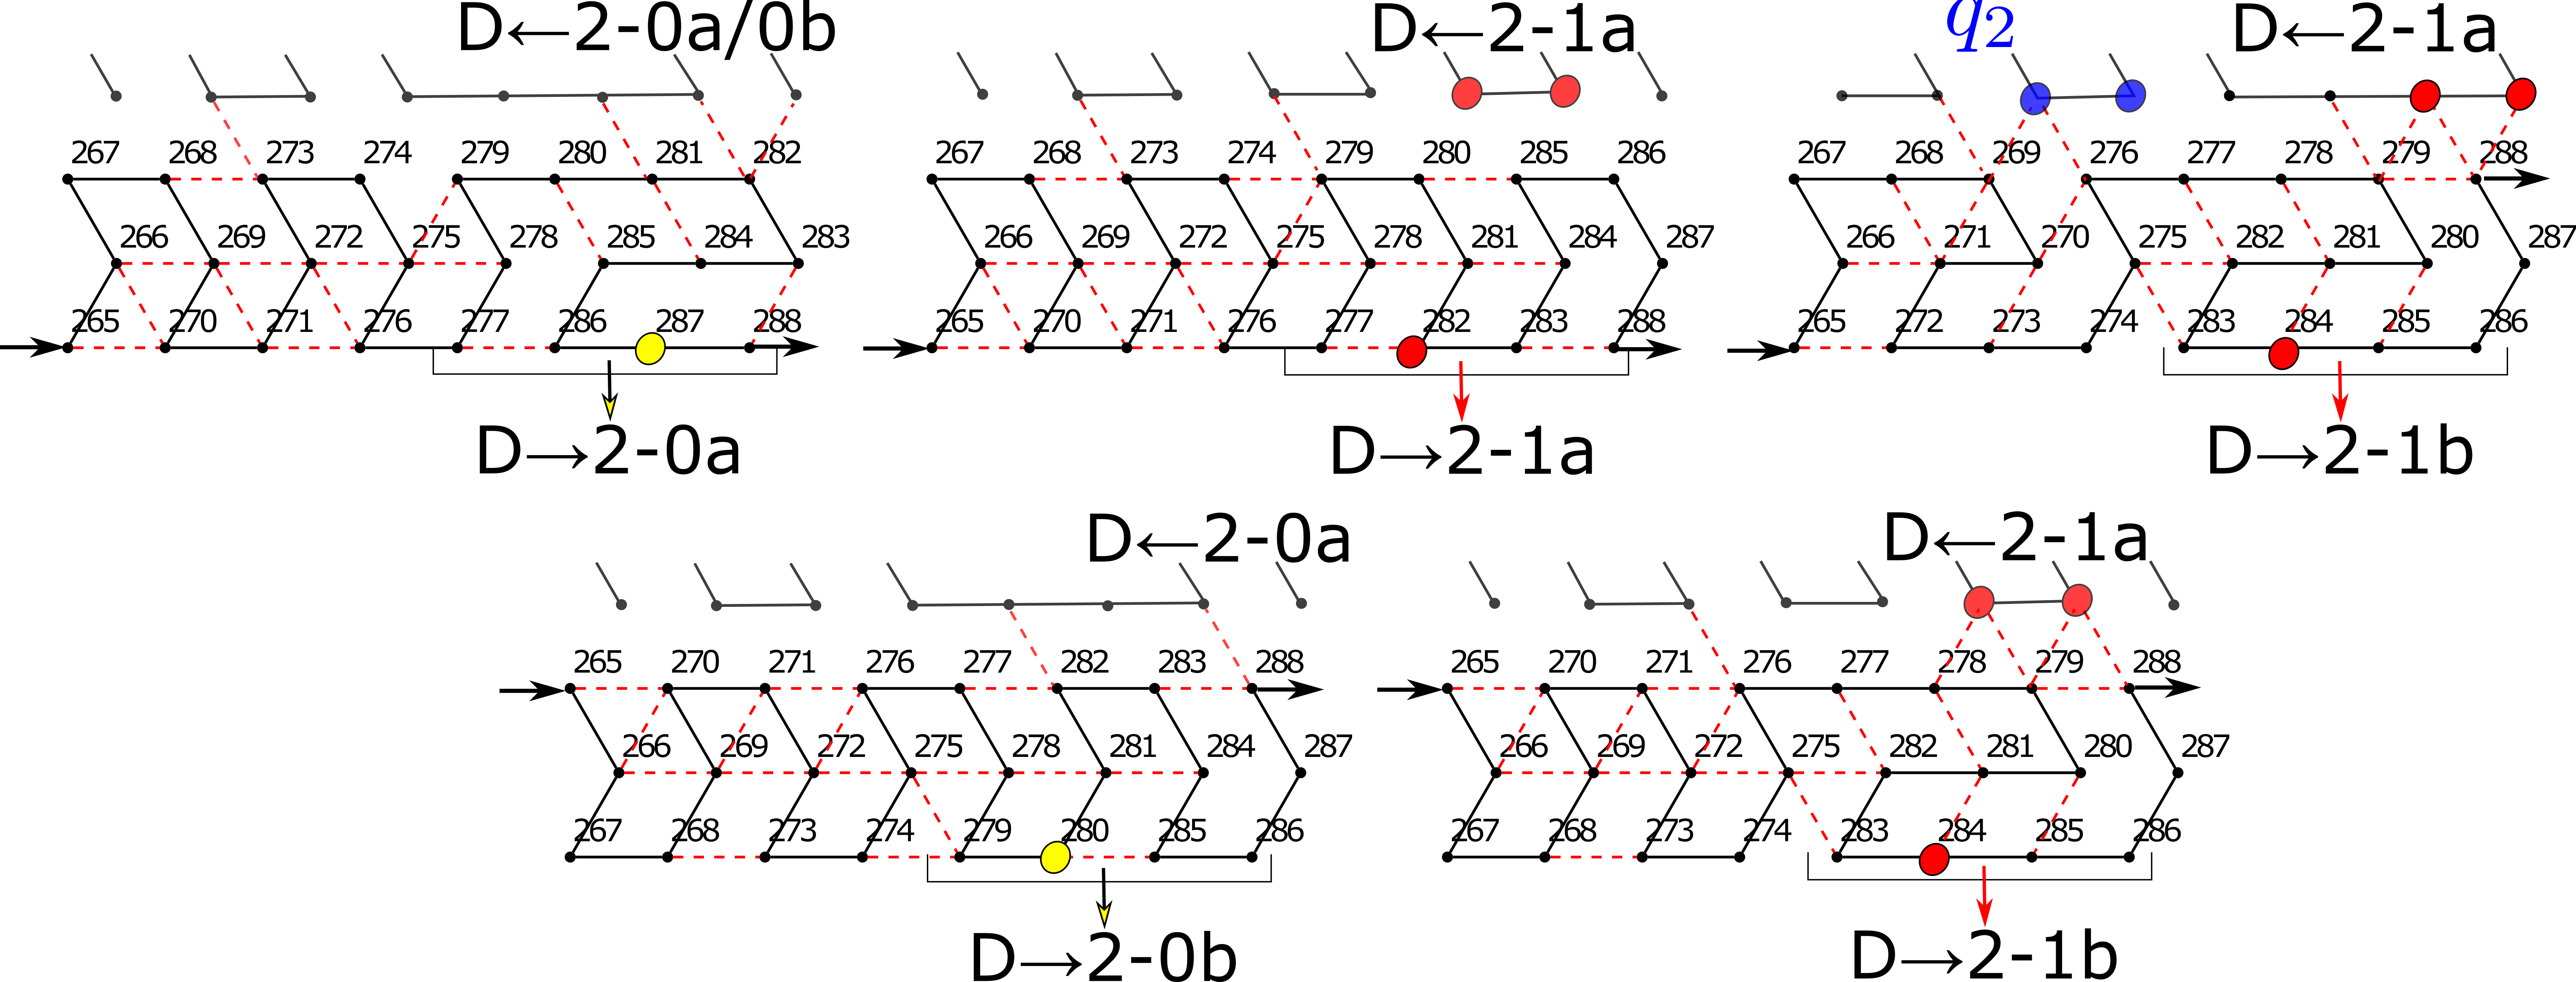
\includegraphics[width=\linewidth]{pic/DFAO-zag2.png}
  \caption{The possible five conformations of DFAO-zag2: (top) Dzag2-L0, Dzag2-L1, Dzag2-T1, (bottom) Dzag2-R0, and Dzag2-R1.}
  \label{fig:DFAO-zag2}
  \end{figure} 
%%%%%%%%%%%%%%%%%%%%%%%%%%%

In the second zig, DFAO-zig2's check whether the first 0 is followed by 0 or 1, being read from LSB.
They first copy all the 1's up to the first 0 by taking the conformation Dzig2-1 (top left in Figure~\ref{fig:DFAO-zig2}).
The next letter is the first 0, which is distinguished from other 0's by the special conformation Dzag1-f0 of the DFAO-zag1 responsible for the bit, or more precisely, by its marker f0. 
Starting at the bottom and reading 0, the DFAO-zig2 can take two conformations Dzig2-0 and Dzig2-f0.
These conformations share the first half.
The marker f0 folds the second half so as to end at the top, yielding Dzig2-f0. 
The next DFAO-zig2 therefore starts to fold at the top so that it takes one of the two conformations Dzig2-f00 and Dzig2-f01 depending on the bit read.
Recall that reading 1 here is equivalent to transitioning to $q_2$, that is, $P[i] = L$.
Observe that Dzig2-f01 is provided with the marker $q_2$, which lets the DFAO-zag2 component below know $P[i] = L$. 
These conformations end at the bottom.
The remaining 0's and 1's are copied by Dzig2-0 and Dzig2-1, respectively.
The second zag starts at the bottom and copy 0's and 1's by the two conformations Dzag2-L0 and Dzag2-L1 of DFAO-zag2 (top left and center in Figure~\ref{fig:DFAO-zag2}) until a DFAO-zag2 encounters a 1, or more precisely, its marker $q_2$, if any. 
Such DFAO-zag2 takes the special conformation Dzag2-T1 and changes the ending position to the top, letting the remaining DFAO-zag2s rather take Dzag2-R0 and Dzag2-R1 for copying, which end at the top.
As such, the second zag can feed $P[i]$ to PFS as explained before, while propagating the current count $i$.

The third zig lets $P[i]$ go through its AO (or $\overline{\rm AO}$) component to be reinterpreted either as A(cute) or as O(btuse) and propagates the current count $i$.   


%%%%%%%%%%%%%%%%%%%%%%%%%%%%%%%
%-------------------------------------------------------------------------------------------
			\subsubsection{Turning module}
%-------------------------------------------------------------------------------------------

\begin{figure}[t]
\centering
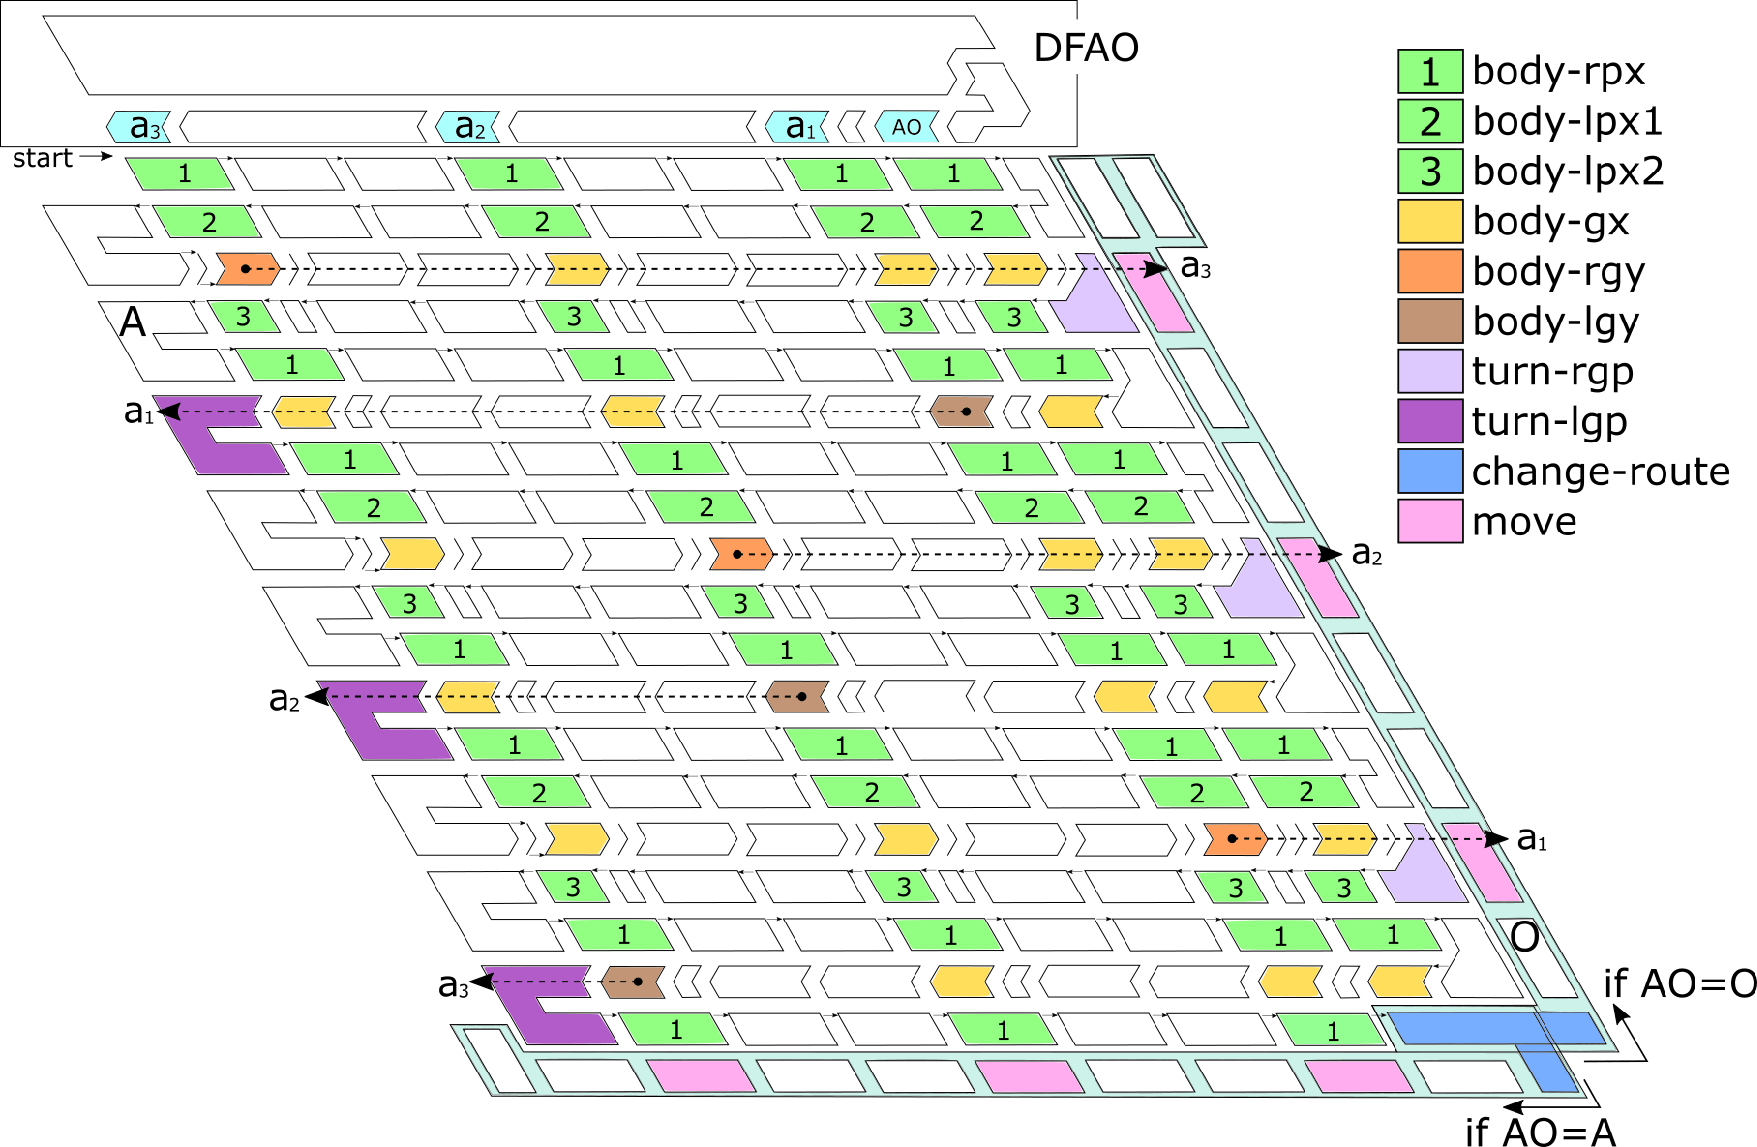
\includegraphics[width=\linewidth]{pic/overall_turn_part.pdf}
\caption{
Component-level abstraction of folding of turning module.
All the white components in the middle are spacers, some of which are implemented in the shape of parallelogram instead of glider. 
 }
\label{fig:overall_turning}
\end{figure}

The last module is for turn. 
It consists of two submodules: bit-sequence bifurcator and steering arm (shaded in light blue in Fig.~\ref{fig:overall_turning}). 

The bifurcator bifurcates the bits of the current count $i$ and the reinterpreted signal (A or O) as shown in Fig.~\ref{fig:abst_dragon} while folding into zigzags.
For that, it employs components to handle the following four types of tasks: 
\begin{enumerate}[itemsep=0pt]
\item propagate 1-bit vertically: body-rpx (Fig.~\ref{fig:body-rpx} (left)), body-lpx1 (Fig.~\ref{fig:body-rpx} (right)), and body-lpx2 (Fig.~\ref{fig:half-adder});
\item let 1-bit cross another 1-bit: body-gx (Fig.~\ref{fig:DFAO-zag2}); 
\item fork 1-bit vertically and horizontally: body-rgy (Fig.~\ref{fig:DFAO-zag2}) and body-lgy (Fig.~\ref{fig:body-lgy});  
\item undergo transition between a zig and a zag and exposes 1-bit outside: turn-rgp (Fig.~\ref{fig:turn-rgp}) and turn-lgp (Fig.~\ref{fig:turn-lgp}). 
\end{enumerate} 
%that propagates 1bit vertically (body-rpx, body-lpx1, and body-lpx2 in Figure~\ref{fig:overall_turning}), that lets 1bit cross another 1bit (body-gx), that forks 1bit vertically and horizontally (body-rgy, body-lgy), and that undergoes transition from a zig to a zag or from a zag to a zig and exposes 1bit outside (turn-rgp, turn-lgp).
Components to handle the first two types of tasks have already been implemented (see, e.g., \cite{HaKiOtSe2016}) so that we shall explain the others.

%The component body-rgy takes one of the two conformations in Figure~\ref{fig:body-rgy} depending on the 1-bit encoded in the two beads above.
%Output below, the 1-bit is encoded as a type of the second bead from left, while output right, it is encoded as the position of its last bead (top or bottom).
%Its zag-variant, body-lgy, is implemented analogously; for its conformations.

%\begin{figure}[h]
\begin{wrapfigure}{r}{0.55\linewidth}
\vspace*{-5mm}
\centering
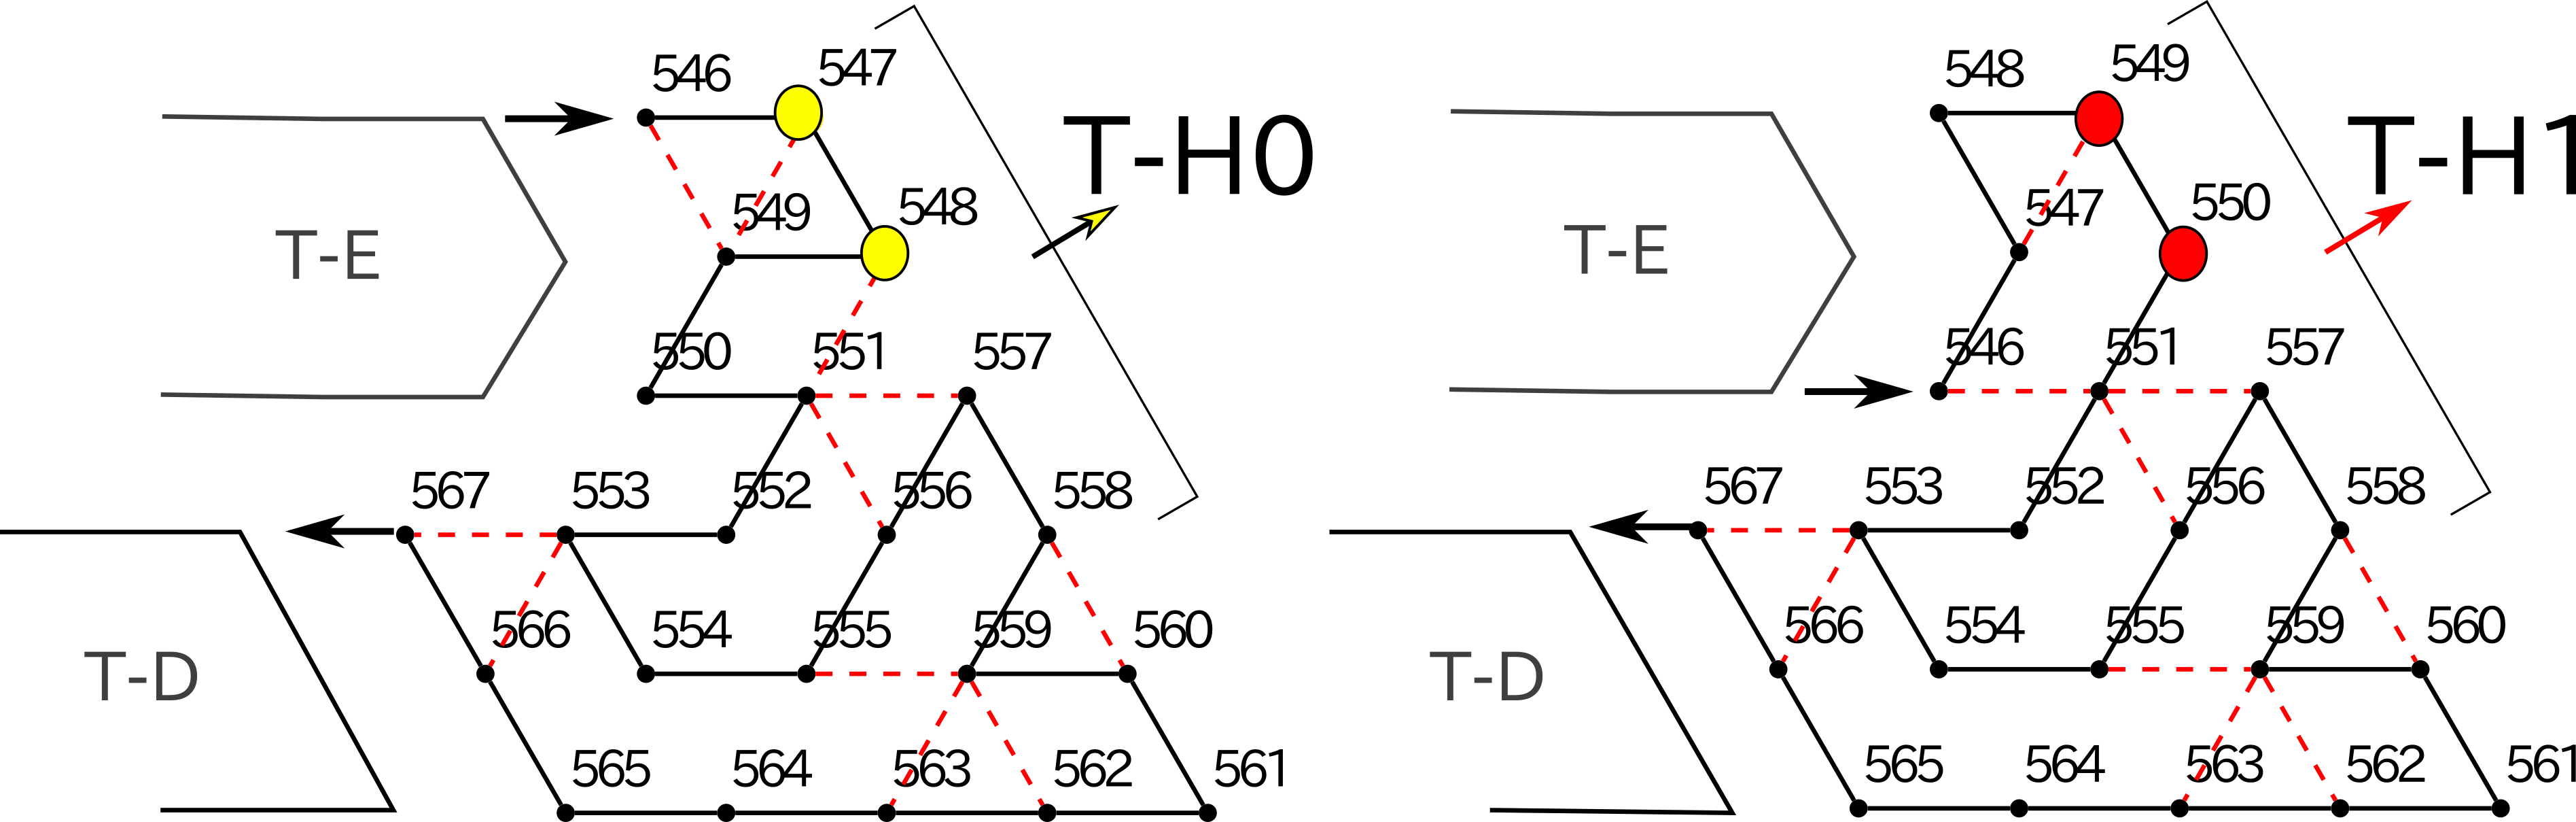
\includegraphics[width=\linewidth]{pic/turn-rgp.png}
\caption{The two conformations of turn-rgp.}
\label{fig:turn-rgp}
\vspace*{-3mm}
\end{wrapfigure}
%\end{figure}

The component body-rgy is implemented by reusing the first half of DFAO-zag2 (Fig.~\ref{fig:DFAO-zag2}). 
Starting from the bottom, it can take two conformations which end at different heights and expose sequences of bead types sufficiently pairwise distinct downward. 
Hence, we can divert it to fork 1bit input rightward and downward. 
The 1bit thus forked transfers till the end of a zag and is converted by the turn-rgp into a sequence of bead types (see Fig.~\ref{fig:turn-rgp}). 
The body-lgy and turn-lgp are their zig counterparts (Figs.~\ref{fig:body-lgy} and \ref{fig:turn-lgp}). 

%The 1bit forked rightward by a body-rgy transfers till the end of the zig without being jammed because all remaining modules in the zig are designed in such a way that they start and end at the same height like the even-distance glider.
%The module turn-rgp receives the 1bit (top or bottom), and exposes it by taking one of the two comformations in Figure~\ref{fig:turn-rgp}.
%The module turn-lgp functions analogously in zags as being folded in Figure~\ref{fig:turn-lgp}.

\begin{figure}[h]
\centering
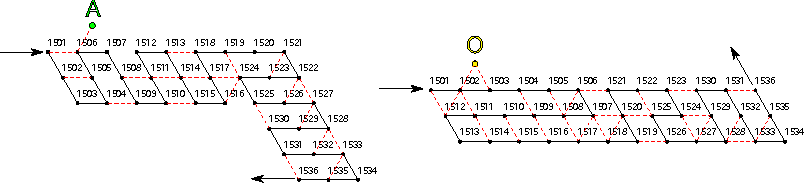
\includegraphics[width=\linewidth]{pic/change_route.pdf}
\caption{The two conformations of change-route.}
\label{fig:change_route}
\end{figure}

The bifurcator also propagates the 1-bit A/O, output by the DFAO module, to tell the steering arm which way it should take.
Specifically, the signal has the component, change-route, of the steering arm take one of the two conformations in Fig.~\ref{fig:change_route}, guiding the rest of the arm towards the specified direction.
The remaining arm is a catenation of move components (Fig.~\ref{fig:move}), which is capable of letting the bifurcated bit sequence through.  
Note that the turning module need not bifurcate AO.
Indeed, the second and third turning modules are supposed to turn in the same manner as the first one.
It hence suffices to append A and O to the bifurcated bit sequences on the acute side and obtuse side, respectively, as shown in Fig.~\ref{fig:overall_turning}.

\begin{remark}
As suggested in Fig.~\ref{fig:overall_turning}, the bifurcation component actually outputs an input bit sequence also downward.
That is, it trifurcates the input.
This provides a more space-efficient way to replicate a bit sequence many-folds.
\end{remark}


%%%%%%%%%%%%%%%%%%%%%%%%%%%%%%%